\section{Introduction, background concepts, decision problems}
\Que{What is a game in game theory?}
\Ans[Game theory]{ is a mathematical framework that allows to model specific type of problems. The problems studied by game theory are called games.}

\Que{What is a game?}
\Ans[A game]{ is a multi-person multi-objective problem.}
\medskip
\small{
\textbf{Multi-person} = There are multiple agents (players) involved in a game

\textbf{Multi-objective} = Players have, in general, different goals

The \textbf{outcome} of a game depends on the choices made by all players

The \textbf{purpose} of game theory is to find the “best choice” for each of them according to their objectives}

\Que{What does it mean for a preference to be rational?}
\Ans[A preference]{ is rational when it's complete and transitive}
\medskip
\small{\textbf{Preference} is a binary relationship $\succeq$ between
elements of \m{A} (set of possible actions)

If \m{a,b \in A, a \succeq b}  means that \m{a} is preferred to \m{b}

A \textbf{preference} is always: reflexive, anti-symmetric
A preference can also be:
\begin{itemize}
    \item \textbf{complete} if \m{\fa a,b \in A} either \m{a \succeq b} or \m{b \succeq a}
    \item \textbf{transitive} if \m{\fa a,b \in A, a \succeq b \wedge b \succeq c \Rightarrow a \succeq c}
\end{itemize}}

\Que{What does it mean for a player to be rational?}
\Ans[A player is rational]{ when he always maximize their utility function, i.e., choose the action that leads to his preferred
outcome. In other words, rational player act for their own good.}

\Que{What are the elements of a decision problem?}
\Ans[A decision problem]{ has three elements: actions, outcomes and preferences.}
\medskip
\small{
\textbf{Action} \m{a} is selected from a set of possible actions \m{A}

Action \m{a} results in a certain \textbf{outcome} (For 1-player problems actions = outcomes)

\textbf{Preferences} describe the relationship between different outcomes (i.e., which one is preferred)}

\Que{How to represent a decision tree?}
\Ans[A decision tree]{ has players on nodes, actions on branches and payoffs on leaves.

\begin{center}
    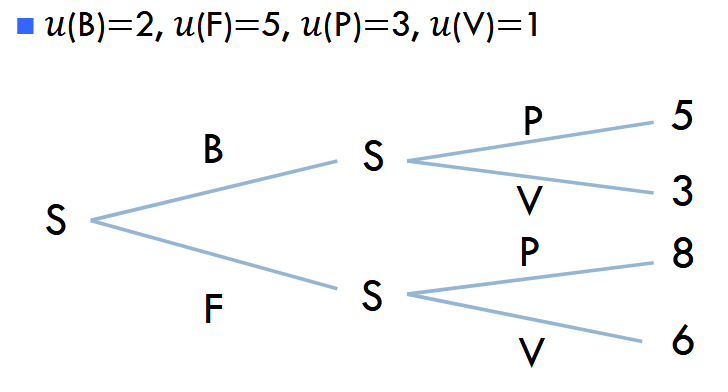
\includegraphics[width=0.5\textwidth]{decTree}
\end{center}}